\documentclass[14pt]{beamer}
%\documentclass[14pt,handout]{beamer}

%\usepackage{pgfpages}
%\pgfpagesuselayout{4 on 1}[letterpaper, border shrink = 10mm, landscape]
%\pgfpagesuselayout{2 on 1}[letterpaper, border shrink = 10mm, portrait]

\mode<presentation> {

% The Beamer class comes with a number of default slide themes
% which change the colors and layouts of slides. Below this is a list
% of all the themes, uncomment each in turn to see what they look like.

%\usetheme{default}
\usetheme{AnnArbor}
%\usetheme{Antibes}
%\usetheme{Bergen}
%\usetheme{Berkeley}
%\usetheme{Berlin}
%\usetheme{Boadilla}
%\usetheme{CambridgeUS}
%\usetheme{Copenhagen}
%\usetheme{Darmstadt}
%\usetheme{Dresden}
%\usetheme{Frankfurt}
%\usetheme{Goettingen}
%\usetheme{Hannover}
%\usetheme{Ilmenau}
%\usetheme{JuanLesPins}
%\usetheme{Luebeck}
%\usetheme{Madrid}
%\usetheme{Malmoe}
%\usetheme{Marburg}
%\usetheme{Montpellier}
%\usetheme{PaloAlto}
%\usetheme{Pittsburgh}
%\usetheme{Rochester}
%\usetheme{Singapore}
%\usetheme{Szeged}
%\usetheme{Warsaw}

% As well as themes, the Beamer class has a number of color themes
% for any slide theme. Uncomment each of these in turn to see how it
% changes the colors of your current slide theme.

%\usecolortheme{albatross}
%\usecolortheme{beaver}
%\usecolortheme{beetle}
%\usecolortheme{crane}
%\usecolortheme{dolphin}
%\usecolortheme{dove}
%\usecolortheme{fly}
%\usecolortheme{lily}
%\usecolortheme{orchid}
%\usecolortheme{rose}
%\usecolortheme{seagull}
%\usecolortheme{seahorse}
%\usecolortheme{whale}
\usecolortheme{wolverine}

%\setbeamertemplate{footline} % To remove the footer line in all slides uncomment this line
%\setbeamertemplate{footline}[page number] % To replace the footer line in all slides with a simple slide count uncomment this line

%\setbeamertemplate{navigation symbols}{} % To remove the navigation symbols from the bottom of all slides uncomment this line
}


%\usepackage{fullpage}
\usepackage[all]{xy}

\usepackage{graphicx}
\usepackage{subfigure}
%\usepackage{float}
%\usepackage{wrapfig}
\usepackage{rotating}

%\usepackage{lscape}
\usepackage{amsmath}
\usepackage{amsfonts}
\usepackage{amssymb}
\usepackage{amsthm}
\usepackage{wasysym}

\usepackage{relsize}
\usepackage{multicol}
\usepackage{multirow}

\usepackage{color}

%\usepackage{cite}
\usepackage{latexsym}


%\usepackage{ulem}
\usepackage{cancel}
\usepackage{enumerate}
%\usepackage{amscd}

%\usepackage[psamsfonts]{eucal}

%\usepackage{listings}

%\usepackage{citesort}
%\usepackage[dvips]{epsfig}
%\usepackage{psfrag}
%\usepackage{indentfirst}
%\usepackage{setspace}




%\usepackage[pdftex]{hyperref}
%\hypersetup{pdfborder={0 0 0 0}}

%\usepackage[margin=1in,paperwidth=8.5in,paperheight=11in]{geometry}


%\usepackage{fancyhdr}
%\pagestyle{fancy}
%\fancyhf{} % clear all header and footer fields
%%%\fancyfoot[R]{Choroszucha\ \thepage}
%\lhead{\nouppercase\leftmark}
%\rhead{{Castro and $\BBC$horoszucha} \thepage}
%\fancyfoot{}
%%\renewcommand{\headrulewidth}{0pt}
%%\renewcommand{\footrulewidth}{0pt}





%\setlength{\paperwidth}{8.5in}
%\setlength{\paperheight}{11in}

%\setlength{\voffset}{-0.5in}
%\setlength{\hoffset}{0in}
%\setlength{\textwidth}{6.5in}%6in
%\setlength{\textheight}{9in}
%\setlength{\oddsidemargin}{0mm}
%\setlength{\evensidemargin}{0mm}
%\setlength{\topmargin}{0in}
%\setlength{\headheight}{0.25in}
%\setlength{\headsep}{0.25in}
%\setlength{\marginparsep}{5mm}
%\setlength{\marginparwidth}{0.75in}
%\setlength{\footskip}{0.25in}


%\setlength\parskip{0.125in}


\usepackage{etex}
%\usepackage{mathabx}
\usepackage{xcolor,colortbl}

\definecolor{Grey}{gray}{0.9}
\definecolor{White}{gray}{1}
%\newcommand\md{\ }
%\DeclareSymbolFont{AMSb}{U}{msb}{m}{n}
%\DeclareMathSymbol{\R}{\mathbin}{AMSb}{"52}
%\DeclareMathSymbol{\Z}{\mathbin}{AMSb}{"5A}
%\DeclareMathSymbol{\Q}{\mathbin}{AMSb}{"51}
%\DeclareMathSymbol{\F}{\mathbin}{AMSb}{"46}
%\DeclareMathSymbol{\C}{\mathbin}{AMSb}{"43}
%\DeclareMathSymbol{\B}{\mathbin}{AMSb}{"42}



\newcommand{\bernNTensor}[2]{\overset{#2\rightharpoonup}{#1}}
\newcommand{\bernMatrix}[1]{\overset{\rightharpoonup}{\overset{\rightharpoonup}{#1}}}
%\newcommand{\bernmatrixfull}[3]{\left.\overset{\rightharpoonup}{\overset{\rightharpoonup}{#1}_{#2}\right|_{#3}}
\newcommand{\bernVector}[1]{\overset{\rightharpoonup}{#1}}
\newcommand{\bernVectorFull}[3]{\left.\overset{\rightharpoonup}{#1}_{#2}\right|_{#3}}

\newcommand{\myHat}[2]{\hat{#1}_{#2}}
\newcommand{\rowVector}[3]{\left[\begin{array}{c} #1\\ #2\\ #3\end{array}\right]}
\newcommand{\columnVector}[3]{\left[\begin{array}{c c c} #1 & #2 & #3 \end{array}\right]}







\newcommand{\boxedeqn}[1]{%
  \[\fbox{%
      \addtolength{\linewidth}{-2\fboxsep}%
      \addtolength{\linewidth}{-2\fboxrule}%
      \begin{minipage}{\linewidth}%
      \begin{equation}#1\end{equation}%
      \end{minipage}%
    }\]%
}


\newcommand{\eulerX}[1]{%
\left[\begin{array}{c c c}
1 & 0 &0\\
0 & \cos\left(#1\right) & \sin\left(#1\right)\\
 0 & -\sin\left(#1\right)& \cos\left(#1\right) 
\end{array}\right]}


\newcommand{\eulerY}[1]{%
\left[\begin{array}{c c c}
\cos\left(#1\right) &0& -\sin\left(#1\right) \\
0 & 1 & 0\\
 \sin\left(#1\right)& 0 &\cos\left(#1\right)
\end{array}\right]}

\newcommand{\eulerZ}[1]{%
\left[\begin{array}{c c c}
\cos\left(#1\right) & \sin\left(#1\right)& 0 \\
 -\sin\left(#1\right)& \cos\left(#1\right)& 0 \\
0 & 0& 1 
\end{array}\right]}

\newcommand{\myNorm}[2]{%
\left\|#1\right\|_{#2}
}

\newcommand{\diag}{{\rm diag}}
\newcommand{\myspan}{{\rm span}}
\newcommand{\Mat}{{\rm Mat}}
\newcommand{\Ker}{{\rm Ker}}
\newcommand{\myImage}{{\rm Im}}



\title[EECS 568]{Multi-Robot/Coordinated SLAM with Particle Filters} % The short title appears at the bottom of every slide, the full title is only on the title page

\author{R Choroszucha, A Collier, and C Hyman}
%\institute[EECS 568] % Your institution as it will appear on the bottom of every slide, may be shorthand to save space
%{
%}
%\date{\today} % Date, can be changed to a custom date
\date{2015-04-20} % Date, can be changed to a custom date

\usepackage{enumerate}
\setlength{\parindent}{0in}


%\begin{frame}
%\frametitle{}
%\end{frame}

\newcommand\blfootnote[1]{%
  \begingroup
  \renewcommand\thefootnote{}\footnote{#1}%
  \addtocounter{footnote}{-1}%
  \endgroup
}
%\setbeamercovered{transparent}
%\setbeamercovered{transparent=20}
%\setbeamertemplate{bibliography item}{}

\usepackage[backend=biber]{biblatex} 
%\usepackage{multimedia}
%\usepackage[3D]{movie15}
%\usepackage{media9}
 
\begin{document}

\begin{frame}
\titlepage % Print the title page as the first slide
\end{frame}


%\begin{frame}
%\frametitle{Overview}
%\tableofcontents 
%\end{frame}

\frame{\frametitle{Overview}\tableofcontents}

\section{Multi-Robot SLAM}
%\frame{\frametitle{Overview}\tableofcontents[currentsection]}
\begin{frame}
\frametitle{Single Robot/Multi-Robot SLAM}
\begin{itemize}
\item Single Robot
\begin{itemize}
\item Very slow to map a large area
\item Increase speed $\rightarrow$ increase noise/decrease accuracy
\item Not robust: single point of failure
\end{itemize}
\item Multi-Robot SLAM (MRSLAM)
\begin{itemize}
\item SLAM with multiple robots searching the space and communicating with each other
\item May still use slower robots
\item May have robot failure, but still achieve mapping objective
%\item Two types:
%\begin{itemize}
%\item Known initial poses
%\item Encounter based
%\end{itemize}
\end{itemize}
\end{itemize}
\end{frame}

\begin{frame}
\frametitle{Challenges of MRSLAM}
\begin{itemize}
\item Often do not know initial poses
\begin{itemize}
\item Need to calculate relative poses
\end{itemize}
\item Complexity 
\begin{itemize}
\item Exploration/Coordination, efficiently move with little overlap and to get as much coverage as possible	
\end{itemize}
\item Each robot is taking measurements in its own frame
\begin{itemize}
\item How to transform the pose data?
\item How to combine the data?
\item How to create a global map?
\end{itemize} 
%\begin{itemize}
%\item 
%\end{itemize}
%\item Encounter based: robots ``observing'' each other

%\item Any portion of a feature/map can correspond, how should the individual maps be merged?
\end{itemize}
\end{frame}


\begin{frame}
\frametitle{Solving MRSLAM}
\begin{itemize}
\item Most papers solve 1 problem at a time
\begin{itemize}
\item Coordination ([Juli{\'a} et. al, 2012])
\item Map Merging ([Lazaro et. al., 2013], [Lee et. al., 2012],[Birk and Carpin, 2006], [Howard, 2006])
\end{itemize}
\item Focus: [Howard, 2006]
\begin{itemize}
\item Answers merging problem
\item All robots store sensor data for both odometry and measurements
\item Starts with a single robot, stored data integrated transformed data into the map posterior post encounter
\item Builds occupancy grid
%\item Transforms relative poses using robot encounter information to create a single map posterior

\end{itemize}

\end{itemize}
\end{frame}


\begin{frame}
\frametitle{MRSLAM Assumptions}
\begin{itemize}
\item Robots move independently of each other
\item Can determine the relative poses of each robot perfectly on an encounter
\item Continued communication post encounter
\item Robot encounters form a connected graph
\begin{center}
\begin{tabular}{cc}
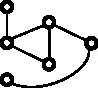
\includegraphics[width=3cm]{../FiguresAndMovies/ConnectedGraph}&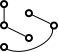
\includegraphics[width=3cm]{../FiguresAndMovies/NonConnected}\\
Connected & Not Connected
\end{tabular}
\end{center}
\end{itemize}
\end{frame}



\begin{frame}
\frametitle{[Howard, 2006] Algorithm}
\begin{itemize}
\item Occupancy Grid FastSLAM 
\item Store $(u_t,z_t,encounter_t)$ data
\item On encounter, replay past data in reverse order
\begin{center}
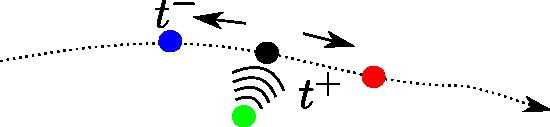
\includegraphics[height=2cm]{../FiguresAndMovies/ForwardBackward}
\end{center}
\item Post encounter integrate stored information into the map posterior in an acausal update
\item Continue communication to integrate future odometry and encounters
\end{itemize}
\end{frame}


\begin{frame}
\frametitle{Causal/Acausal Updates}
\begin{center}
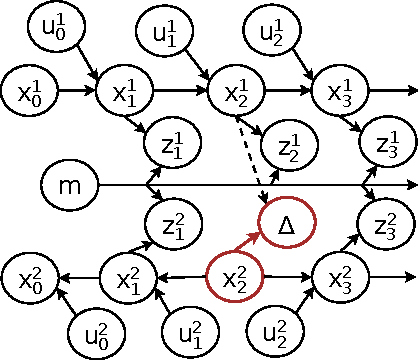
\includegraphics[height=6cm]{../FiguresAndMovies/HowardFig3}
\end{center}
\blfootnote{From [Howard, 2006]}
\end{frame}

\begin{frame}
\frametitle{[Howard, 2006] Algorithm}
\begin{itemize}
\item Robot 1 observes robot 2
\end{itemize}
\begin{center}
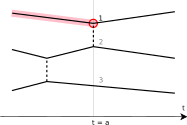
\includegraphics[height=5cm]{../FiguresAndMovies/Howard5a}
\end{center}
\blfootnote{From [Howard, 2006]}
\end{frame}


\begin{frame}
\frametitle{[Howard, 2006] Algorithm}
\begin{itemize}
\item Robot 2 observes robot 3, integrating robot 3 data
\end{itemize}
\begin{center}
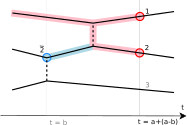
\includegraphics[height=5cm]{../FiguresAndMovies/Howard5b}
\end{center}
\blfootnote{From [Howard, 2006]}
\end{frame}

\begin{frame}
\frametitle{[Howard, 2006] Algorithm}
\begin{itemize}
\item Data is propagated, now all data is used for map
\end{itemize}
\begin{center}
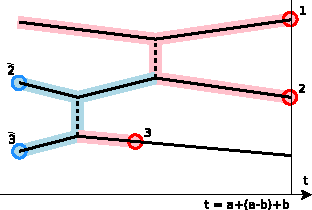
\includegraphics[height=5cm]{../FiguresAndMovies/Howard5c}
\end{center}
\blfootnote{From [Howard, 2006]}
\end{frame}




\section{Experimental Validation}
%\frame{\frametitle{Overview}\tableofcontents[currentsection]}
\begin{frame}
\frametitle{The Tests}
\begin{tabular}{cc}
\hspace{-0.75cm}\begin{minipage}{0.5\textwidth}
\begin{itemize}
\item Occupancy Grid
\begin{itemize}
\item Custom Map
\item m robots
\end{itemize}
\end{itemize}
\end{minipage} & \hspace{-0.75cm}\begin{minipage}{0.6\textwidth}

\includegraphics[width=\textwidth]{../FiguresAndMovies/Test5}
\end{minipage}
\end{tabular}
\end{frame}

\begin{frame}
\frametitle{Validation}
%\movie[width=5cm,poster]{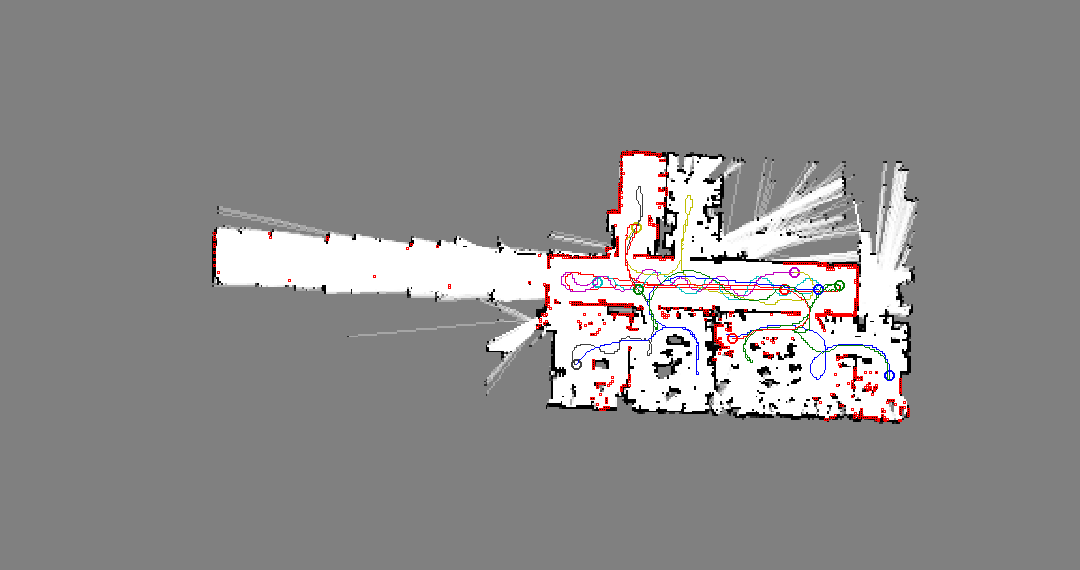
\includegraphics[width=5cm]{{{../FiguresAndMovies/gridmap_416-10}}}}{../FiguresAndMovies/20150416T220508-gridmap-10.mp4}

%\includemovie[autoplay, poster]{4cm}{3cm}{../FiguresAndMovies/20150416T220508-gridmap-10.mp4}

%\includemedia[
%  label=vidB,
%  addresource=../FiguresAndMovies/20150416T220508-gridmap-10.mp4,
%  activate=pageopen,
%  width=5cm, height=4cm,
%  flashvars={
%     source=../FiguresAndMovies/20150416T220508-gridmap-10.mp4
%    &loop=true
%  }
%]{}{VPlayer.swf}


\begin{center}
\href{run:../FiguresAndMovies/20150416T220508-gridmap-10.mp4}{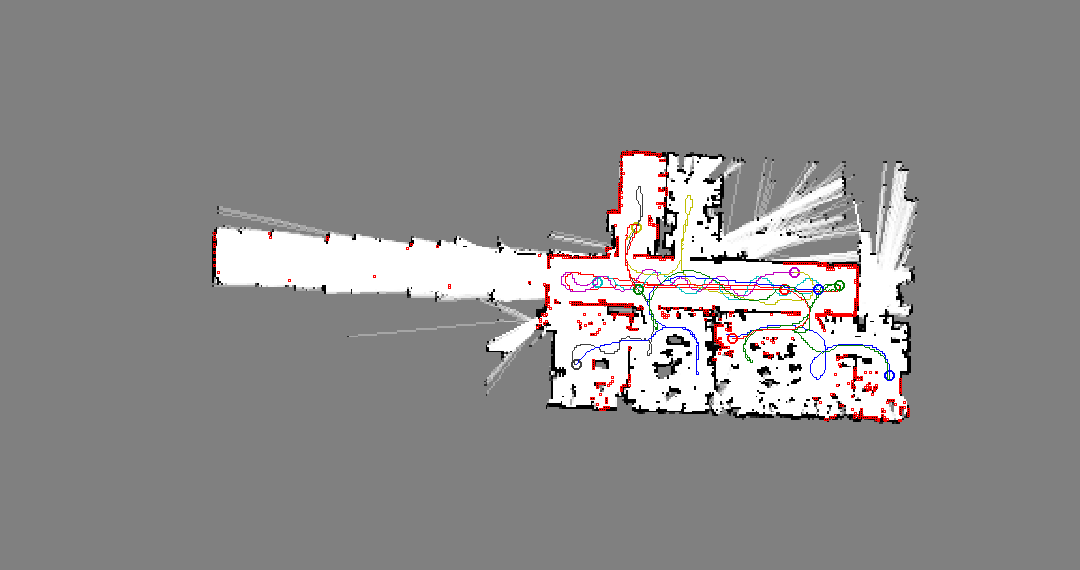
\includegraphics[width=12cm]{{{../FiguresAndMovies/gridmap_416-10}}}}
\end{center}
\end{frame}


%\section{Nonlinear MPC Simulation Question}
%\frame{\frametitle{Overview}\tableofcontents[currentsection]}

\section{Conclusions and Future Work}
%\frame{\frametitle{Overview}\tableofcontents[currentsection]}
\begin{frame}
\frametitle{Conclusions}
\begin{itemize}
\item Conclusions:
\begin{itemize}
\item 
\end{itemize}
\item Future work:
\begin{itemize}
\item Decrease 
\item Make it work on Albert B data set
\end{itemize}
\end{itemize}
\end{frame}


%\begin{frame}[allowframebreaks]
%\nocite{*}
%        \frametitle{References}
%        \bibliographystyle{plain}
%        %\bibliography{../../Journal/Citations-MPCConstraintTightening}
%        \bibliography{Citations-MPCConstraintTightening}
%\end{frame}

\begin{frame}[t]
\nocite{*}
        \frametitle{References}
        %\vspace{-0.5cm}
        %\tiny{\bibliographystyle{abbrv}}
        %\bibliography{../../Journal/Citations-MPCConstraintTightening}
        %\bibliography{Citations-Prospectus.bib}
        \tiny{\frametitle<presentation>{Further Reading}    

  \begin{thebibliography}{10}    
%  \beamertemplatebookbibitems
  \setbeamertemplate{bibliography item}[text]
%  \beamertemplatearticlebibitems

%  \bibitem{WangBoyd}
%	Y. Wang and S. Boyd.
%	\newblock {\em “Fast model predictive control using online optimization.”}
%	\newblock IEEE Transactions on Control Systems Technology, 18(2). 2010.

%  \bibitem{}
%    \newblock 
%    \newblock 



\bibitem{julia2012comparison}
	M.~Juli{\'a}, A.~Gil, and O.~Reinoso
    \newblock {\em ``A comparison of path planning strategies for autonomous exploration and mapping of unknown environments.''}
    \newblock Autonomous Robots, 2012.  

  \bibitem{6696483}
	M.T.~Lazaro, L.M.~Paz, P.~Pinies, J.A.~Castellanos, and G.~Grisetti
    \newblock {\em ``Multi-robot SLAM using condensed measurements.''}
    \newblock International Conference on Intelligent Robots and Systems, 2013.  

  \bibitem{lee2012probabilistic}
	H.C.~Lee, S.H.~Lee, M.H.~Choi, and B.H.~Lee
    \newblock {\em ``Probabilistic map merging for multi-robot RBPF-SLAM with unknown initial poses.''}
    \newblock Robotica, 2012.  

  \bibitem{birk2006merging}
	A.~Birk, and S.~Carpin.
    \newblock {\em ``Merging occupancy grid maps from multiple robots.''}
    \newblock Proceedings of the IEEE, 2006.  

  \bibitem{howard2006multi}
	A.~Howard.
    \newblock {\em ``Multi-robot simultaneous localization and mapping using particle filters.''}
    \newblock The International Journal of Robotics Research, 2006.  


  \bibitem{thrun2005probabilistic}
    S.~Thrun, W.~Burgard, and D.~Fox
    \newblock {\em ``Probabilistic Robotics.''}
    \newblock MIT press, 2005.    



    


       
    
    
  \end{thebibliography}}
		%\printbibliography 
\end{frame}

\begin{frame}
\frametitle{}
\begin{center}
{ \Huge Questions...}
\end{center}
\end{frame}

%\section*{Extra}
%
%\begin{frame}
%\frametitle{}
%\begin{center}
%{ \Huge Extra Slides}
%\end{center}
%\end{frame}
%
%\input{Extra}



\end{document}


%\lstset{
%basicstyle=\tiny,
%keywordstyle=\color{blue},
%commentstyle=\color{green},
%stringstyle=\ttfamily,
%numbers=left,
%}